%\documentclass[german,10pt]{book}      
\usepackage{makeidx}
\usepackage{babel}            % Sprachunterstuetzung
\usepackage{amsmath}          % AMS "Grundpaket"
\usepackage{amssymb,amsfonts,amsthm,amscd} 
\usepackage{mathrsfs}
\usepackage{rotating}
\usepackage{sidecap}
\usepackage{graphicx}
\usepackage{color}
\usepackage{fancybox}
\usepackage{tikz}
\usetikzlibrary{arrows,snakes,backgrounds}
\usepackage{hyperref}
\hypersetup{colorlinks=true,
                    linkcolor=blue,
                    filecolor=magenta,
                    urlcolor=cyan,
                    pdftitle={Overleaf Example},
                    pdfpagemode=FullScreen,}
%\newcommand{\hyperref}[1]{\ref{#1}}
%
\definecolor{Gray}{gray}{0.80}
\DeclareMathSymbol{,}{\mathord}{letters}{"3B}
%
\newcounter{num}
\renewcommand{\thenum}{\arabic{num}}
\newenvironment{anmerkungen}
   {\begin{list}{(\thenum)}{%
   \usecounter{num}%
   \leftmargin0pt
   \itemindent5pt
   \topsep0pt
   \labelwidth0pt}%
   }{\end{list}}
%
\renewcommand{\arraystretch}{1.15}                % in Formeln und Tabellen   
\renewcommand{\baselinestretch}{1.15}                 % 1.15 facher
                                                      % Zeilenabst.
\newcommand{\Anmerkung}[1]{{\begin{footnotesize}#1 \end{footnotesize}}\\[0.2cm]}
\newcommand{\comment}[1]{}
\setlength{\parindent}{0em}           % Nicht einruecken am Anfang der Zeile 

\setlength{\textwidth}{15.4cm}
\setlength{\textheight}{23.0cm}
\setlength{\oddsidemargin}{1.0mm} 
\setlength{\evensidemargin}{-6.5mm}
\setlength{\topmargin}{-10mm} 
\setlength{\headheight}{0mm}
\newcommand{\identity}{{\bf 1}}
%
\newcommand{\vs}{\vspace{0.3cm}}
\newcommand{\noi}{\noindent}
\newcommand{\leer}{}

\newcommand{\engl}[1]{[\textit{#1}]}
\parindent 1.2cm
\sloppy

         \begin{document}  \setcounter{chapter}{8}


\chapter{Die Kosmische Entfernungsleiter}
% Kap 9
\label{chap_Kosm_Entfernung}

\info{Thomas Filk}{28.03.2024}%
Die Bestimmung astronomischer bzw.\ kosmischer Entfernungen ist sowohl ein
spannendes Thema der Geschichte der Physik als auch ein interessantes
Forschungsfeld der modernen Physik. W\"ahrend der Abstand von der Erde zum
Mond schon im Altertum bekannt war (siehe Abschnitte \ref{sec_Aristarchos} und \ref{sec_Eratosthenes}) 
kennt man den Abstand von der Erde zur Sonne -- die sogenannte Astronomische
Einheit AU (astronomical unit) -- mit einer gewissen Verl\"asslichkeit erst seit dem 18.\ Jahrhundert.

Tabelle \ref{tab_Arist} enth\"alt einige Daten, die in diesem Abschnitt gelegentlich
verwendet werden.\index{Abstand!Erde-Sonne}\index{Abstand!Erde-Mond}\index{AU - Astronomische Einheit}%
\index{Erddurchmesser}\index{Monddurchmesser}\index{Sonne!Durchmesser}

\begin{table}[htb]
\begin{tabular}{l|c|l}
Bezeichnung & Symbol & Wert \\ \hline
Durchmesser Erde & $D_{\rm E}$ &  $D_{\rm E}= 12\,740\,{\rm km}$ \\
Durchmesser Mond & $D_{\rm M}$ &  $D_{\rm M}= 3\,474\,{\rm km}$ \\
Durchmesser Sonne & $D_{\rm S}$ &  $D_{\rm S}=  1\,400\,000 \,{\rm km}$ \\
Abstand Erde-Mond & $r_{\rm M}$  &  $r_{\rm M} = 380\,000\,{\rm km}$ \\
Abstand Erde-Sonne & $r_{\rm S}$  &  $r_{\rm S} = 150\,000\,000\,{\rm km}$ \\
Winkel Sonne-Mond bei Halbmond & $\alpha$ & $\alpha = 89^\circ 51'$ \\ \hline
\end{tabular}
\caption{\label{tab_Arist}%
Einige Daten des Sonne-Erde-Mond-Systems.}
\end{table}

\section{Aristarchos von Samos}
\label{sec_Aristarchos}

Aristarchos von Samos\index{Aristarchos von Samos} 
lebte um 310\,v.Chr. bis 230\,v.Chr, also kurz nach Aristoteles (384-322 v.Chr.)
und ungef\"ahr zeitgleich mit Archimedes (284-212\,v.Chr.). Er stellte sich die Sonne als ein riesiges
Himmelsfeuer vor, das unter anderem den Mond anstrahlt. Er deutete eine Mondfinsternis
korrekt als ein Ereignis, bei dem sich die Erde zwischen Sonne und Mond schiebt und dadurch
auf dem Mond der Erdschatten sichtbar wird. Au\ss erdem deutete er den Halbmond als das Ereignis,
bei dem die Verbindungslinie Sonne-Mond senkrecht zur Verbindungslinie Erde-Mond steht. Aus diesen
beiden Interpretationen sowie den zugeh\"origen Messungen konnte er \textit{relative} Gr\"o\ss en
bestimmen: das Verh\"altnis der Abst\"ande Erde-Mond zu Erde-Sonne, das Verh\"altnis Monddurchmesser zu
Sonnendurchmesser, das Verh\"altnis Monddurchmesser zu Erddurchmesser und schlie\ss lich
konnte er daraus das Verh\"altnis der Gr\"o\ss e der Sonne zur Gr\"o\ss e der Erde bestimmen. Seine
Schlussfolgerung war, dass die Sonne wesentlich gr\"o\ss er sein muss als die Erde, und damit sollte
seiner Meinung nach die Sonne im Zentrum des Universums stehen. Dadurch wurde er einer der ersten
Vertreter eines heliozentrischen Weltbilds.

\begin{figure}[htb]
\begin{tikzpicture}
\draw (1,1.5) circle (1.6cm);
\draw (9.3,1.5) circle (0.15cm);
\draw (10.6,1.5) circle (0.4cm);
\draw (1,-0.1) -- (10.2,1.5);
\draw (1,3.1) -- (10.2,1.5);
\draw (1,-0.1) -- (14,1.5);
\draw (1,3.1) -- (14,1.5);
\filldraw[fill=gray!20] (14,1.5) -- (10.6,1.1) arc (270:440:0.4cm) -- (14,1.5);
\draw (11.9,1.5) circle (0.15cm);
\draw (11.83,1.07) circle (0.15cm);
\draw (1,-0.1) -- (1,3.1);
\draw (1.3,1.5) node{$D_{\rm S}$}; 
\draw (10.6,1.1) -- (10.6,1.9);
\draw (10.8,1.5) node{${\scriptstyle D_{\rm E}}$}; 
\draw (8.7,1.5) node{\footnotesize Mond}; 
\draw (1,-0.5) -- (10.6,-0.5);
\draw (1,-0.6) -- (1,-0.4);
\draw (10.6,-0.6) -- (10.6,-0.4);
\draw (6.3,-0.27) node{$r_{\rm S}$}; 
\draw (9.3,0.0) -- (10.6,0.0);
\draw (9.3,-0.1) -- (9.3,0.1);
\draw (10.6,-0.1) -- (10.6,0.1);
\draw (9.8,0.18) node{$r_{\rm M}$}; 
\draw (10.6,-0.25) -- (14.0,-0.25);
\draw (10.6,-0.35) -- (10.6,-0.15);
\draw (14,-0.35) -- (14,-0.15);
\draw (12.3,-0.05) node{$R$}; 
\draw (14.2,1.245) -- (14.2,1.755);
\draw (14.1,1.245) -- (14.3,1.245);
\draw (14.1,1.755) -- (14.3,1.755);
\draw (14.4,1.5) node{$B$}; 
\filldraw[fill=black!100] (11.88,1.755) circle (0.03cm);
\filldraw[fill=black!100] (11.88,1.245) circle (0.03cm);
\draw (10.6,1.5) circle (1.3cm);
\draw (9.6,1.75) node{\tiny (1)}; 
\draw (12.17,1.05) node{\tiny (2)}; 
\draw (12.25,1.5) node{\tiny (3)}; 
\end{tikzpicture}
\caption{\label{fig_Arist}%
Nicht ma\ss stabsgetreue Verh\"altnisse zwischen Sonne, Mond und Erde. Es sind drei
Mondphasen dargestellt: (1) Der Mond bei einer Sonnenfinsternis, er erscheint genauso gro\ss\ wie die
Sonne; (2) der Mond tritt in den Erdschatten und (3) der Mond befindet sich
im Erdschatten. $R$ bezeichnet die L\"ange des Erdschattens und $B$ seine Breite an der Stelle
des Monddurchgangs.}
\end{figure}

In vereinfachten Rechnungen nimmt man gelegentlich an, dass der Erdschatten beim Mond denselben Durchmesser
hat wie die Erde. Das setzt voraus, dass die Sonne \glqq unendlich\grqq\ weit entfernt ist, sodass der 
Erdschatten durch nahezu paralleles Sonnenlicht entsteht. Diese Annahme konnte Aristarchos aber 
nicht machen: Erstens wollte er ja erst zeigen, dass die Sonne sehr weit von der Erde entfernt ist,
und zweitens war der relative Abstand, den er aus seinen Messungen erhielt, um einen Faktor 20
kleiner als in Wirklichkeit. Au\ss erdem steht eine solche Annahme in einem (etwas versteckten) Widerspruch 
zu einer in die Rechnungen eingehenden Beobachtung und f\"uhrt zu
einem deutlichen Fehler, wie gegen Ende dieses Abschnitts gezeigt wird. 

Statt dessen nahm Aristarchos an, dass sich der Erdschatten hinter der Erde wie ein Kegel
verj\"ungt und daher der Mond bei einer Mondfinsternis einen kleineren Schattendurchmesser 
durchl\"auft, als es dem Erddurchmesser entspricht (siehe Abb.\ \ref{fig_Arist}). Um diese 
Verj\"ungung des Erdschattens ber\"ucksichtigen 
zu k\"onnen, musste er erst bestimmen, wie weit die Sonne von der Erde relativ zum Mond entfernt ist.

\begin{figure}[htb]
\begin{tikzpicture}
\draw (1,1.5) circle (1.0cm);
\draw (10.5,2.8) circle (0.15cm);
\draw (10.6,1.5) circle (0.4cm);
\draw (1,1.5) -- (10.5,2.8) -- (10.6,1.5) -- (1,1.5);
\draw (10.6,1.4) node{\footnotesize Erde}; 
\draw (11.1,2.8) node{\footnotesize Mond}; 
\draw (1,1.4) node{\footnotesize Sonne}; 
\draw (10.45,1.65) node{${\scriptstyle \alpha}$};
\filldraw[fill=black!100] (10.35,2.55) circle (0.03cm);
\draw (10,2.75) arc (185:275:0.5cm);
\draw (6,1.3) node{$r_{\rm S}$};
\draw (10.85,2.15) node{$r_{\rm M}$};
\filldraw[fill=gray!50] (10.52,2.65) arc (278:458:0.15cm);
\end{tikzpicture}
\caption{\label{fig_Arist2}%
Der Mond bei Halbmond. Der Winkel, unter dem vom Mond aus betrachtet die Zentren von
Sonne und Erde erscheinen, betr\"agt $90^\circ$. Der Winkel, unter dem von der Erde
aus betrachtet die Zentren von Sonne und Mond erscheinen ist $\alpha$. Der Kosinus von $\alpha$ entspricht 
dem Verh\"altnis von den Abst\"anden Erde-Mond zu Erde-Sonne.}
\end{figure}

F\"ur die Bestimmung der relativen Entfernung der Sonne ging Aristarchos von folgender 
\"Uberlegung aus: Bei Halbmond ist der Winkel zwischen der Verbindungslinie Sonne-Mond
und der Verbindungslinie Erde-Mond ein rechter Winkel (siehe Abb.\ \ref{fig_Arist2}). Wenn man nun hier auf der
Erde den Winkel $\alpha$ zwischen den Verbindungslinien Erde-Sonne und Erde-Mond 
bestimmt, erh\"alt man das Verh\"altnis der Abst\"ande von Erde-Sonne zu Erde-Mond.
Heute w\"urden wir daf\"ur schreiben:
\begin{equation}
\label{eq_Arist1}
                     \frac{r_{\rm M}}{r_{\rm S}} = \cos \alpha \, . 
\end{equation} 
Allerdings erhielt Aristarchos f\"ur diesen Winkel mit $\alpha = 87^\circ$ einen viel zu kleinen Wert.
Der tats\"achliche Wert ist $89^\circ 51'$. Vermutlich war sich Aristarchos dar\"uber im Klaren, dass
der Wert f\"ur $\alpha$ kleiner als $90^\circ$ sein muss und sein Wert ist eher als eine
untere Grenze zu verstehen. 
Mit dem Wert von Aristarchos ist der Abstand Sonne-Erde
rund 19 mal gr\"o\ss er als der Abstand Erde-Mond. In Wirklichkeit ist das Verh\"altnis knapp 400. 
Da die Sonne von der Erde aus betrachtet \"ahnlich gro\ss\ erscheint wie der Mond (bei einer
Sonnenfinsternis wird die Sonne vom Mond gerade eben bedeckt), ist die Sonne um dasselbe
Verh\"altnis gr\"o\ss er als der Mond - f\"ur Aristarchos rund 19 mal gr\"o\ss er. Das bedeutet:
\begin{equation}
\label{eq_Arist2}
                           \frac{D_{\rm S}}{D_{\rm M}} = \frac{r_{\rm S}}{r_{\rm M}} \, .
\end{equation}

Aus Abbildung \ref{fig_Arist} erhalten wir die folgenden geometrischen Beziehungen (in beiden F\"allen
aus dem Strahlensatz):
\begin{equation}
\label{eq_Arist3}
        \frac{D_{\rm S}}{D_{\rm E}} = \frac{R+r_{\rm S}}{R} =  1+\frac{r_{\rm S}}{R}  \hspace{1.0cm} {\rm und} \hspace{1cm}
        \frac{B}{D_{\rm E}} = \frac{R-r_{\rm M}}{R} =  1-\frac{r_{\rm M}}{R}  \, .
\end{equation}
Eine weitere Beziehung erhielt Aristarchos aus der Messung von zwei Zeitdauern: 
$t_1$ sei die Zeitdauer zwischen dem Moment, in dem der Mond in den Schatten der Erde eintritt, bis
zu dem Moment, wo er sich ganz im Erdschatten befindet, und $t_2$ sei die Zeitdauer, in der sich der Mond 
vollst\"andig im Erdschatten befindet. 
Das Verh\"altnis dieser beiden Zeiten ist
\begin{equation}
\label{eq_Arist4}
           \frac{t_1}{t_2} = \frac{D_{\rm M}}{B-D_{\rm M}}   \hspace{1.0cm} {\rm oder} \hspace{1.0cm}
             B= \frac{t_1+t_2}{t_1} D_{\rm M} \, .
\end{equation}
Aus den beiden Beziehungen in Gl.\ \ref{eq_Arist3} k\"onnen wir die L\"ange $R$ des Erdschattens eliminieren,
die Breite $B$ des Erdschattens bei der Mondbahn k\"onnen wir durch Gl.\ \ref{eq_Arist4} ersetzen und
schlie\ss lich k\"onnen wir noch den Sonnendurchmesser $D_{\rm S}$ mit Hilfe von Gl.\ \ref{eq_Arist2} 
durch den Monddurchmesser $D_{\rm M}$ und das bekannte Verh\"altnis $\frac{r_{\rm S}}{r_{\rm M}}$ ersetzen.
Nach einer etwas l\"angeren Rechnung erhalten wir dann:
\begin{equation}
\label{eq_Arist5}
             \frac{D_{\rm E}}{D_{\rm M}} 
             = \frac{\displaystyle \left( 1 + \frac{t_1+t_2}{t_1} \right)}{\displaystyle 1 + \frac{r_{\rm M}}{r_{\rm S}}} \, .
\end{equation}
Auf der rechten Seite stehen nur Gr\"o\ss en, die Aristarchos gemessen hatte. 
Aus seinen Beobachtungen schloss er,
dass die Erde ungef\"ahr 3 mal gr\"o\ss er ist als der Mond (sein Wert war 2,85, der wirkliche Wert
ist 3,67). Zusammen mit seinem Faktor 19 zwischen der Gr\"o\ss e des Monds und der
Gr\"o\ss e der Sonne erhielt er somit, dass die Sonne rund $6,7$ mal gr\"o\ss er sein muss als die
Erde. Der wirkliche Faktor ist knapp 110. 

\begin{SCfigure}[30][htb]
\begin{tikzpicture}
\draw (0,0) node{\mbox{~}};
\draw (8.5,0) node{\mbox{~}};
\draw (2.5,1) node{${\scriptstyle \theta}$};
\draw (8.3,1) node{${\scriptstyle D_{\rm M}}$};
\draw (5,0.85) node{${\scriptstyle r_{\rm M}}$};
\draw (0.2,1) -- (2.3,1);
\draw (2.7,1) -- (8,1);
\draw (0.2,1) -- (8,0.5) -- (8,1.5) -- (0.2,1) ;
\draw[thick] (8.02,0.5) -- (8.02,1.5);
\draw (2.6,0.84) arc (351:369:1.0); 
\end{tikzpicture}
\caption{\label{fig_Arist3}%
Aus dem \"Offnungswinkel, unter dem der Mond von der Erde aus gesehen wird (ungef\"ahr $30'$) kann man auf
das Verh\"altnis von Monddurchmesser $D_{\rm M}$ zum Abstand Erde-Mond $r_{\rm M}$ schlie\ss en.}
\end{SCfigure}

Dar\"uber hinaus konnte Aristarchos
aus der scheinbaren Gr\"o\ss e des Monds (ungef\"ahr $0,5^\circ$ \"Offnungswinkel) das
Verh\"altnis von der Gr\"o\ss e des Monds $D_{\rm M}$ zu seinem Abstand $r_{\rm M}$ 
von der Erde bestimmen (siehe Abb.\ \ref{fig_Arist3}).
Die Beziehung ist:
\begin{equation}
\label{eq_Parallaxe}
                       \tan \frac{\theta}{2} = \frac{D_{\rm M}}{2 r_{\rm M}} \, .
\end{equation}  

H\"atten wir f\"ur die Breite $B$ des Erdschattens beim Mond einfach den Erddurchmesser
angenommen, h\"atten wir direkt aus Gl.\ \ref{eq_Arist4} die Beziehung
\begin{equation}
                  \frac{D_{\rm E}}{D_{\rm M}}  = \frac{t_1+t_2}{t_1}    
\end{equation}  
erhalten. Doch
dieses Ergebnis folgt nicht, wenn wir in Gl.\ \ref{eq_Arist5} den Grenzfall $r_{\rm S} \rightarrow \infty$ 
nehmen. Immerhin ist in Wirklichkeit das Verh\"altnis $r_{\rm M}/r_{\rm S}\approx 1/400$ und somit in guter
N\"aherung vernachl\"assigbar. Der zus\"atzliche Term \glqq $1+$\grqq\ im Z\"ahler von Gl.\ \ref{eq_Arist5} r\"uhrt 
ebenfalls daher, dass wir einen kegelartigen Schatten angenommen haben, der an der Stelle des Monds schon 
deutlich kleiner ist als der Erddurchmesser. Wenn $r_{\rm S}$ im Vergleich zu $r_{\rm M}$ gro\ss\ wird, muss
wegen Gl.\ \ref{eq_Arist2}, die wir bei der Herleitung von Gl.\ \ref{eq_Arist5} verwendet haben, auch der
Sonnendurchmesser im selben Verh\"altnis zunehmen. Das bedeutet aber, dass die Schattenl\"ange
$R$ nahezu konstant bleibt (die Korrektur hierzu wird durch den Nenner von Gl.\ \ref{eq_Arist5} beschrieben)
und damit auch das Verh\"altnis, um das der Erdschatten beim Mond kleiner ist. F\"ur das Erde-Sonne-Mond-System
ist $R$ ungef\"ahr das Vierfache von $r_{\rm M}$, und damit ist der Erdschatten beim Mondabstand schon
um ungef\"ahr den Faktor 3:4 kleiner als der Erddurchmesser.  

\section{Eratosthenes von Kyrene}
\label{sec_Eratosthenes}

Wie wir gesehen haben, hat Aristarchos nur Verh\"altnisse von Gr\"o\ss en bestimmt, keine
absoluten Werte. Dazu muss mindestens eine der Gr\"o\ss en bekannt sein. 
Dieses\index{Eratosthenes von Kyrene}
Problem l\"oste Eratosthenes von Kyrene, der kurz nach Aristarchos lebte. Seine genauen
Lebensdaten sind nicht bekannt, aber bis auf ein oder zwei Jahre lebte er von 276\,v.Chr.\ bis
194\,v.Chr. Bekannt ist Eratosthenes unter anderem durch das gleichnamige \glqq Sieb\grqq, mit dem man 
eine Tabelle der Primzahlen erh\"alt. 

Eratosthenes wusste, dass es in der N\"ahe von Assuan (damals Syene) einen tiefen Brunnen
gab, bei dem die Sonne nur einmal im Jahr -- am 21.\ Juni zur Mittagszeit 
(d.h.\ bei Sonnenh\"ochststand) -- den Boden beleuchtete. Er deutete dies 
als die Tatsache, dass an diesem Tag die Sonne senkrecht \"uber Assuan steht. Assuan liegt am
24.\ Breitengrad und somit nur wenig \"uber dem Sommerwendekreis der Sonne (bei $23,5^\circ$). 
Weiterhin nahm Eratosthenes an, dass die Stadt Alexandria auf demselben L\"angengrad wie
Assuan liegt, was nicht ganz richtig ist: Alexandria liegt rund $3^\circ$ weiter westlich. Dieser
Winkel ist jedoch klein genug, um in die
folgenden \"Uberlegungen nur unwesentlich einzugehen. 
Schlie\ss lich wusste Eratosthenes noch, dass der Schatten eines Obelisken in Alexandria zur
Mittagszeit des 21.\ Juni unter einem Winkel von $1/50$.tel eines Vollkreises (also $\theta=7,2^\circ$) fiel. 
Aus der Annahme, dass die Sonnenstrahlen parallel einfallen, konnte er daraus 
schlie\ss en, dass der Erdumfang das 50-fache des Abstands von Alexandria nach Syene 
betr\"agt. 

\begin{SCfigure}[30][htb]
\begin{tikzpicture}
\draw (0,0) node{\mbox{~}};
\filldraw[fill=black!100] (0.5,1.4) circle (0.05cm);
%\draw (0.5,1.4) circle (2cm);
\draw (1.92,0) arc (315:358:2);
\draw (2.5,1.45) arc (363:420:2);
\draw (2.5,1.45) -- (2,1.45) -- (2,1.35) -- (2.5,1.35);
\draw (2.34,2.1) -- (2.82,2.3) -- (2.79,2.35) -- (2.31,2.16);
\draw (0.5,1.4) -- (2.0,1.4);
\draw (2.79,2.35) -- (2.21,2.35);
\draw (2.21,2.35) -- (0.5,1.4);
\filldraw[fill=gray!30] (2.21,2.35) -- (2.33,2.16) -- (2.79,2.35) -- (2.21,2.35);
\draw[->] (8,1.4) -- (4,1.4);
\draw[->] (8,2.3) -- (4,2.3);
\draw (2.7,2.7) node{${\scriptstyle \theta}$};
\draw (1.1,1.4) arc (0:26:0.7);
\draw[->]  (2.6,2.6) arc (160:193:0.5);
\draw (0.9,1.5) node{${\scriptstyle \theta}$};
\draw (2.65,1.2) node{\footnotesize S};
\draw (2.2,2.0) node{\footnotesize A};
\draw (7,1.85) node{\footnotesize Sonne};
\end{tikzpicture}
\caption{\label{fig_Erat}%
Zur Bestimmung des Erdumfangs nach Eratosthenes. Am 21.\ Juni steht die Sonne
mittags senkrecht \"uber einem Brunnen in Syene (S). Zum gleichen Zeitpunkt wirft ein
Obelisk in Alexandria (A) einen Schatten unter dem Winkel $\theta$. Unter demselben
Winkel erscheinen Syene und Alexandria vom Erdmittelpunkt aus betrachtet.}
\end{SCfigure}  

Wie er den Abstand zwischen Alexandria und Syene bestimmt hat, ist nicht genau bekannt. Es gilt aber als wahrscheinlich,
dass er k\"onigliche Schrittz\"ahler eingesetzt hat, diesen Abstand zu messen. Das Ergebnis
waren 5000 Stadien. Es ist auch nicht bekannt, welche Einheit f\"ur ein Stadion Eratosthenes
verwendet hat (es waren damals mehrere Einheiten gebr\"auchlich), vermutlich aber handelte
es sich um eine Einheit nahe bei 160\,m.\footnote{Das mesopotamische Stadion betrug 148,5\,m, das
griechische 177,6\,m. In manchen griechischen Schriften findet man auch 157,5\,m.} 
In diesem Fall h\"atte er die Entfernung Alexandria-Syene 
nach heutigen Einheiten zu 800\,km bestimmt. Da dies 1/50.\ des Erdumfangs entsprechen
soll, bestimmte er den Erdumfang zu 40\,000\,km. Wie genau diese Werte mit seinen Werten
\"ubereinstimmen, ist nicht bekannt, aber immerhin handelte es sich um ein wissenschaftliches
Verfahren, wohingegen viele andere Werte f\"ur die Gr\"o\ss e der Erde auf reinen Vermutungen beruhten. 

\section{Die Gr\"o\ss e der Erde}

Bis in die fr\"uhe Neuzeit wurden die antiken Ergebnisse zur Bestimmung der Gr\"o\ss e
der Erde oder des Abstands Erde-Sonne kaum \"ubertroffen. Die Zahlen von Eratosthenes
blieben obskur, solange nicht gekl\"art war, was genau unter einem Stadion zu verstehen war.
Doch die allgemeine Idee zur Bestimmung der Gr\"o\ss e der Erde war korrekt. 

Zu Beginn des 17.\ Jahrhunderts gab es zwei Entdeckungen, die einen wesentlichen
Fortschritt brachten: (1) die Erfindung des Fernrohrs um 1610 und (2) die Kepler'schen Gesetze,
insbesondere das dritte Kepler'sche Gesetz, das eine Beziehung zwischen den gro\ss en Halbachsen
und den Umlaufzeiten eines Planeten um die Sonne herstellte (ver\"offentlicht 1619). 

Mit Hilfe des Fernrohrs konnte die Erdgr\"o\ss e wesentlich genauer bestimmt werden. Hier ist
insbesondere\index{Picard, Jean} 
Jean Picard (1620--1682) zu erw\"ahnen, der um 1670 eine sehr genaue Vermessung
des Erdradius vornahm. Voraussetzung daf\"ur waren (1) die Festlegung von zwei 
m\"oglichst weit voneinander entfernten Orten auf demselben L\"angengrad, (2) eine 
m\"oglichst genaue Bestimmung der Entfernung zwischen diesen beiden Orten und (3) eine
m\"oglichst genaue Messung der Breitengrade dieser Orte. Picard verwendete zur Winkelmessung
zwischen zwei Orten Quadranten, die mit kleinen Fernrohren mit Fadenkreuzen ausgestattet
waren. Dadurch waren sehr pr\"azise Winkelmessungen m\"oglich. Diese verwendete er einerseits,
um den Breitengrad beispielsweise durch Sternbeobachtungen genau zu bestimmen, andererseits
konnte er \"uber\index{Triangulatioin} 
Triangulationen\footnote{Von zwei Punkten aus, deren Abstand bekannt ist, wird
ein dritter Punkt anvisiert und es werden die beiden Winkel zwischen dem jeweils anderen Punkt
und dem dritten Punkt vermessen. Daraus lassen sich die Entfernungen der beiden Punkte zu
dem dritten Punkt bestimmen. Zur Kontrolle kann man von diesem dritten Punkt aus den Winkel zu
den beiden Ausgangspunkten bestimmen. Jean Picard entdeckte auf diese Weise, dass Licht
an unterschiedlichen Luftschichten -- z.B.\ unterschiedlich bez\"uglich ihrer Temperatur oder ihres
Drucks -- gebrochen wurde.} 
die Entfernungen zwischen zwei Punkten ausmessen, sofern
die L\"ange einer Basislinie bekannt war. Durch weitere Anwendung dieses Verfahrens kann man
auch gr\"o\ss ere Abst\"ande bestimmen. Letztendlich gen\"ugt die Kenntnis einer Basislinie, um
\"uber genaue Winkelmessungen gro\ss e Entfernungen ausmessen zu k\"onnen. Ob sich zwei
Orte genau auf demselben L\"angengrad befinden, konnte man dadurch feststellen, dass man
von einem erh\"ohten Punkt (Geb\"aude, H\"ugel oder Bergspitze) exakt zur Mittagszeit (definiert
durch den lokalen Sonnenh\"ochststand, der die Richtung \glqq S\"uden\grqq\ anzeigt) 
jeweils einen Punkt im S\"uden und einen im Norden anvisierte. 

Picard erreichte eine Genauigkeit von ungef\"ahr $0,1$\% f\"ur seine Bestimmung des Erdradius.
Nachdem im 18.\ Jahrhundert mehrere solche Messungen an verschiedenen Orten der Erde
durchgef\"uhrt worden waren, erkannte man, dass die Erde keine exakte Kugelform hat. Gleiche
Breitengradunterschiede hatten in Poln\"ahe einen gr\"o\ss eren Abstand als in \"Aquatorn\"ahe, was auf
die Form eines abgeplatteten Ellipsoids schlie\ss en lie\ss. 

\section{Der Abstand Erde-Sonne}

Die Idee der Parallaxenmessung wird in\index{Parallaxe}
Abb.\ \ref{fig_Parallaxe} verdeutlicht. Beobachtet man ein Objekt $S$ von zwei verschiedenen
Punkten $a$ und $b$ aus, deren Abstand $D$ bekannt ist, kann man aus dem Winkel $\alpha$,
um den dieses Objekt verschoben zu sein scheint, die Entfernung zu $S$ bestimmen. 
Es wird dabei die Formel \ref{eq_Parallaxe} verwendet. Vor einem \glqq unendlich weit\grqq\ entfernten
Hintergrund kann man den Winkel $\alpha$ sehr leicht bestimmen, indem man den Winkel zwischen den 
scheinbaren Orten $A$ und $B$ des Objekts vor dem Hintergrund ausmisst. 
Nach einem \"ahnlichen Verfahren bestimmen wir intuitiv mit unseren Augen den Abstand von
Gegenst\"anden, wobei $D$ dem Abstand der Augen entspricht.

\begin{figure}[htb]
\begin{tikzpicture}
\draw (0.3,0) -- (0.3,3);
\draw (14.2,0.5) -- (14.2,2.5);
\filldraw[fill=black!100] (11.34,1.5) circle (0.05); 
\filldraw[fill=black!100] (14.2,1.2) circle (0.05); 
\filldraw[fill=black!100] (14.2,1.8) circle (0.05); 
\filldraw[fill=black!100] (0.3,0.34) circle (0.05); 
\filldraw[fill=black!100] (0.3,2.66) circle (0.05); 
\draw (12.4,1.38) arc (350:370:0.7);
\draw (10.3,1.62) arc (170:190:0.7);

\draw (12.4,1.37) arc (168:192:0.7);
\draw (12.4,1.92) arc (168:192:0.7);

\draw (14.2,1.2) -- (0.3,2.66);
\draw (14.2,1.8) -- (0.3,0.34);
\draw (0.3,2.66) -- (14.2,1.8);
\draw (0.3,0.34) -- (14.2,1.2);
\draw (12.2,1.5) node{${\scriptstyle \alpha}$};
\draw (10.5,1.5) node{${\scriptstyle \alpha}$};
\draw (12.6,1.23) node{${\scriptstyle \beta}$};
\draw (12.6,1.75) node{${\scriptstyle \beta}$};
\draw (0.1,0.34) node{${\scriptstyle B}$};
\draw (0.1,2.66) node{${\scriptstyle A}$};
\draw (14.35,1.2) node{${\scriptstyle a}$};
\draw (14.35,1.8) node{${\scriptstyle b}$};
\draw (11.34,1.7) node{${\scriptstyle S}$};
\draw (14.35,1.5) node{${\scriptstyle D}$};
\end{tikzpicture}
\caption{\label{fig_Parallaxe}%
Die Parallaxenmessung. Beobachtet man ein Objekt $S$ von zwei verschiedenen Orten $a$ und $b$
aus, so erscheint dieser Gegenstand um den Winkel $\alpha$ verschoben. Die beiden Richtungen 
$A$ und $B$ erscheinen von $a$ bzw.\ $b$ aus unter dem Winkel $\beta$. Vor einem \glqq unendlich weit\grqq\
entfernten Hintergrund gilt $\alpha=\beta$. Kennt man den Abstand $D$ zwischen den Punkten $a$ und $b$,
kann man aus dem Winkel $\alpha$ den Abstand zu $S$ bestimmen. Selbst wenn $A$ und $B$ nicht
unendlich weit entfernt sind, wie bei der Parallaxe der Venus vor der Sonne, kann man aus der Kenntnis
der relativen Abst\"ande und dem gemessenen Winkel $\beta$ den Winkel $\alpha$ bestimmen.}
\end{figure}

Eines der Hauptargumente in der Antike gegen das heliozentrische Weltbild des Aristarchos war 
das Fehlen jeglicher Parallaxen. Das bezog sich einerseits auf das Fehlen von Parallaxen der 
Planeten -- wie beispielsweise des Mars, dem erdn\"achsten Planeten, den wir gegen einen Nachthimmel 
beobachten k\"onnen --, wobei hier der Erdradius den Ma\ss stab f\"ur den Abstand setzt
unter dem eine Parallaxe beobachtet wird. Andererseits bezog sich das aber auch auf die 
fehlende Parallaxe der Sterne,
wobei hier der Radius der Erdumlaufbahn um die Sonne diesen Ma\ss stab setzt. Doch schon
Archimedes hatte in einem Kommentar zu Aristarchos in seinem 
\textit{Sandrechner} die\index{Sandrechner (Archimedes)}
zu gro\ss en Abst\"ande zwischen den Himmelsk\"orpern f\"ur die nicht beobachteten Parallaxen 
verantwortlich gemacht.\footnote{Er hatte im \textit{Sandrechner}
explizit angenommen, dass sich der Abstand der Sterne zum Abstand Erde-Sonne \"ahnlich verh\"alt
wie der Abstand Erde-Sonne zum Durchmesser der Erde. Damit brachte er zum Ausdruck, dass
der Abstand Erde-Sonne zum Durchmesser der Erde zu gro\ss\ f\"ur eine Parallaxenmessung
der Sonne von der Erde aus ist, und entsprechend der Abstand der Sterne zu gro\ss, um
im Verlauf eines Jahres von verschiedenen Punkten der Erdbahn aus beobachtet zu werden.}  

Grunds\"atzlich war die Idee von Aristarchos zur Bestimmung des Verh\"altnisses $r_{\rm M}/r_{\rm S}$
richtig, es setzt aber voraus, dass man den Winkel zwischen Mond und Sonne bei
Halbmond genau messen kann. Die Fehler beruhen sowohl auf der Bestimmung
des Zeitpunkts, wann genau Halbmond ist, als auch auf der exakten Messung des Winkels, der sehr 
nahe bei $90^\circ$ liegt. Kleine Messfehler f\"uhren hier zu gro\ss en Unsicherheiten, sodass
\"ahnliche Messungen in den Folgezeiten keine wesentlich besseren Ergebnisse erbrachten.
Erst um 1635 wurde die Messung von Godefroy Wendelin nach dem Verfahren von Aristarchos
mit einem Fernrohr wiederholt, was zu\index{Wendelin, Godefroy} 
etwas besseren Werten f\"uhrte: Er bestimmte den Abstand Erde-Sonne zu ungef\"ahr 90\,000\,000\,km.

\"Ahnlich wie schon bei Aristarchos waren die relativen Abst\"ande in unserem Sonnensystem
sp\"atestens seit den Kepler'schen Gesetzen sehr gut bekannt. Das dritte Kepler'sche 
Gesetz\index{Kepler'sches Gesetz!drittes} 
stellt eine Beziehung zwischen den Umlaufzeiten der Planeten und ihren
gro\ss en Halbachsen her, und die Umlaufzeiten lie\ss en sich sehr genau bestimmen. 
Allerdings bezieht sich das dritte Kepler'sche Gesetz auf denselben Zentralk\"orper 
(der Faktor zwischen dem Quadrat der Umlaufzeit und der dritten Potenz der Halbachse
einer Bahn h\"angt von der Masse des Zentralk\"orpers ab), sodass man aus den 
Umlaufzeiten und Halbachsen beispielsweise der Mondbahn nicht auf die entsprechenden
Gr\"o\ss en bei den Planetenbahnen schlie\ss en konnte. Immerhin wusste man nun, dass
man lediglich eine absolute Entfernung im Planetensystem bestimmen musste, um alle
anderen Entfernungen zwischen den Planeten und der Sonne bzw.\ den Planeten
untereinander ebenfalls zu kennen. 

Im 17.\ Jahrhundert wurden mit Hilfe des Fernrohrs Versuche unternommen, aus einer Parallaxenmessung 
des Mars die Entfernung Mars-Erde bei deren Minimum zu bestimmen. Damit h\"atte man auch
den Abstand Sonne-Erde gekannt.\index{Richter, Jean}\index{Cassini, Domenico} 
Jean Richter und Giovanni Domenico Cassini erhielten auf diese
Weise einen Wert f\"ur die Astronomische Einheit, der immerhin schon weniger als 10\% vom
tats\"achlichen Wert abwich. Auf einen \"ahnlichen Wert kam auch\index{Flamsteed, John} 
John Flamsteed. Im Gegensatz zu
Richter und Cassini, die die Mars-Parallaxe von Orten auf zwei verschiedenen Breitengraden
vornahmen (Paris und Cayenne in Franz\"osisch Guayana, knapp \"uber dem \"Aquator), nahm
Flamsteed die Messung alleine vor, indem er die Parallaxe zwischen Abend und Morgen beobachtete und
somit die Drehung der Erde ausnutzte (da sich die Erde in dieser Zeit um eine
unbekannte Distanz weiter um die Sonne bewegte, wobei diese Distanz wiederum nur \"uber
den Abstand Erde-Sonne bestimmt werden konnte, wurde die Rechnung etwas komplizierter). 

1639 fand ein Venus-Transit vor der Sonne statt, den Jeremiah Horrocks nutze, um eine
Parallaxenmessung der Venus vor der Sonne zu messen. Er erhielt einen \"ahnlichen Wert wie
Wendelin mit einem Fehler von rund 40\%. 

Edmund Halley\index{Halley, Edmund}\index{Venus-Transit} 
(basierend auf Arbeiten von James Gregory) hatte 1716 in einem Artikel
gezeigt, dass eine Beobachtung einer Venus-Parallaxe vor der Sonne zu genaueren Ergebnissen
f\"uhren k\"onnte, wenn man nicht die Parallaxenwinkel direkt ausmisst, sondern die Zeiten misst,
f\"ur die die Venus vor der Sonnenscheibe sichtbar ist. Aus diesen Zeitdauern kann
der Winkel $\alpha$ der Parallaxe bestimmt werden. Die Tatsache, dass die Sonne nicht
unendlich weit entfernt ist und insofern die beobachtete Parallaxe vor der Sonne nicht gleich dem
Parallaxenwinkel ist, macht das Problem nicht wesentlich komplizierter, da man aus den
Kepler'schen Gesetzen das Verh\"altnis der Abst\"ande kannte und daraus die richtige Parallaxe
berechnen konnte (Abb.\ \ref{fig_Venus}). 

\begin{figure}[htb]
\begin{tikzpicture}
\draw (2,2) circle (1.5);
\draw (14,2) circle (0.5);
\filldraw[fill=black!100] (9.7,2.2) circle (0.06); 
\filldraw[fill=black!100] (13.6,1.7) circle (0.05); 
\filldraw[fill=black!100] (13.6,2.3) circle (0.05); 
\filldraw[fill=black!100] (11,5) circle (0.07); 
\draw (13.6,1.7) -- (3.1,3);
\draw (13.6,2.3) -- (3.5,2);
\draw (11,2.13) node{${\scriptstyle \alpha}$};
\draw (2,2) node{\footnotesize Sonne};
\draw (14,2) node{\footnotesize Erde};
\draw (9.7,2.4) node{\footnotesize Venus};
%
\draw (9.7,5) circle (2);
\draw (13.0,5) circle (0.02);
\draw (8,7) -- (12,6);
\draw (8,6.95) -- (12,5.94);
\draw[->] (11.5,4) arc (240:180:1);
\draw (9.7,5) node{\footnotesize Sonne};
\draw (13,4.8) node{\footnotesize Erde};
\draw (12.7,4.0) node{\footnotesize Scheinbare Gr\"o\ss e};
\draw (12.7,3.7) node{\footnotesize der Venus vor};
\draw (12.7,3.4) node{\footnotesize der Sonne};
\end{tikzpicture}
\caption{\label{fig_Venus}%
Die Parallaxenmessung bei einem Venus-Transit vor der Sonne. (unten) Die Verh\"altnisse sind \"ubertrieben
dargestellt. Halley hatte vorgeschlagen, von zwei verschiedenen Orten auf der Erde die
genauen Zeiten zu messen, f\"ur die die Venus vor der Sonne sichtbar ist. (oben) Bis auf den Abstand
Sonne-Erde sind hier die Gr\"o\ss en ungef\"ahr ma\ss stabsgetreu dargestellt.
Die Parallaxe der Venus vor der Sonne ist winzig und die scheinbaren Trajektorien
der Venus vor der Sonne liegen sehr dicht beieinander, selbst wenn man sie von weit
entfernten Orten auf der Erde beobachtet. Obwohl die Venus einen etwas kleineren Durchmesser hat
als die Erde, erscheint sie vor der Sonne gr\"o\ss er, da sie sich n\"aher an der Erde befindet.}
\end{figure}

Die tats\"achlichen Verh\"altnisse sind jedoch so, dass diese Zeiten mit einer sehr gro\ss en
Genauigkeit bestimmt werden m\"ussen, da die Venus-Trajektorien vor der Sonnenscheibe
sehr dicht beieinander liegen (Abb.\ \ref{fig_Venus}, oben). Der Winkelabstand der beiden
Trajektorien ist kleiner als der Winkelabstand f\"ur den scheinbaren (projizierten) Durchmesser der Venus. 
Damit ist auch der Zeitpunkt schwer definierbar, wann genau die Venus in den Bereich der Sonnenscheibe 
eintritt oder diesen verl\"asst (eine zus\"atzliche Problematik hierbei ist das sogenannte 
Tropfenph\"anomen:\index{Tropfenph\"anomen}
Aufgrund der endlichen Aufl\"osung optischer Ger\"ate scheint die Venus am inneren Rand der Sonne 
mit dem dunklen Hintergrund tropfenf\"ormig zu verschmelzen).

In den Jahren 1761 und 1769 gab es Venus-Transite, und in diesen Jahren fanden Expeditionen
statt, um die Venus-Parallaxe zu beobachten -- die wichtigste im Jahr 1769, unter anderem mit James
Cook in Tahiti am 17,6-ten s\"udlichen Breitengrad. Der n\"ordlichste 
Beobachtungsort war Vard\o\ am 70-sten n\"ordlichen Breitengrad in Norwegen. Insgesamt gab es bei
den beiden Venus-Transiten weit \"uber einhundert Beobachtungen, verteilt \"uber die ganze Welt. 
Die Daten wurden von\index{Lalande, J\'{e}r\^{o}me} 
J\'{e}r\^{o}me Lalande zusammengetragen und ausgewertet. Der Fehler in der
Bestimmung des Abstands Erde-Sonne betrug letztendlich weniger als 2\%. 

Heute ist die Astronomische Einheit definiert als die\index{AU - Astronomische Einheit} 
L\"ange $1\,{\rm AU}=149\,597\,870\,700$\,m. 
Da die Sonne jedoch st\"andig an Energie und damit Masse verliert, entfernen sich die Planeten
von der Sonne (die Erde um rund 15\,cm im Jahr). Daher wird der Sinn f\"ur eine derart festgelegte
Konstante gelegentlich angezweifelt. 

\section{Parallaxenmessung der n\"achsten Sterne}

Mit der Astronomischen Einheit sind nicht nur die Abst\"ande der Planeten zur Sonne bzw.\ der
Planeten untereinander sowie vieler weiterer Objekte in unserem Sonnensystem bestimmt, sondern damit
steht auch eine neue Basis f\"ur die Messung von Parallaxen zu weiter entfernten Objekten zur
Verf\"ugung. W\"ahrend man insbesondere in der popul\"arwissenschaftlichen Literatur das Lichtjahr 
gerne als astronomische Entfernungseinheit verwendet, also
die Distanz, die das Licht in einem Jahr zur\"ucklegt, verwendet man in der Astrophysik eher
das Parsec, die Parallaxensekunde (abgek\"urzt pc), als Entfernungseinheit. 

Bei einer Geschwindigkeit von 300\,000\,km pro Sekunde ben\"otigt das Licht rund 500\,Sekunden
von der Sonne bis zur Erde, das entspricht 8 Minuten und 20 Sekunden. In einem Jahr legt das
Licht eine Strecke von $9,4673\cdot 10^{12}$\,km zur\"uck. Das ist somit die Distanz, die einem 
Lichtjahr entspricht -- ungef\"ahr $10^{13}$ Kilometer.\index{Parsec, Parallaxensekunde} 
Eine Parallaxensekunde ist definiert als
der Abstand, bei dem die Astronomische Einheit, also der Radius der Erdbahn um die Sonne, 
unter einem Winkel von 1\,Bogensekunde gesehen wird. Eine Bogensekunde sind $1/3600$\,Grad,
und f\"ur eine Parallaxensekunde erhalten wir 
$1\,{\rm pc}=1\,{\rm AU}/\tan (1/3600) \approx 30,857\cdot 10^{12}$\,km. 
Das entspricht $3,26$\,Lichtjahren.   

Der n\"achste Stern (nach der Sonne) ist Proxima Centauri\index{Proxima Centauri} 
mit einem Abstand von $4,25$\,ly (Lichtjahren). 
Hierbei handelt es sich um einen Roten Zwerg, der mit blo\ss em Auge oder auch einem Fernglas
nicht sichtbar ist. Im Abstand von rund $4,38$\,ly ist Alpha-Centauri,\index{alpha@$\alpha$ Centauri} 
einer der hellsten Sterne am Himmel. 
Eigentlich handelt es sich um ein Doppelsternsystem, bestehend aus Alpha-Centauri A und Alpha-Centauri B, 
die jedoch nur mit einem Fernglas oder Fernrohr trennbar sind. Diese Objekte sind also schon weiter
als eine Parallaxensekunde von der Erde entfernt und somit bedarf es sehr hochaufl\"osender 
Teleskope, um die Entfernung zu diesen Sternen mit dem Verfahren der Parallaxe bestimmen zu k\"onnen.
Die erste Ver\"offentlichung einer solchen Messung stammt aus dem Jahre 1838, als Friedrich Wilhelm
Bessel\index{Bessel, Friedrich Wilhelm} 
die Entfernung von Cygni-61\index{Cygni-61} 
(einem bei guten Bedingungen mit blo\ss em Auge sichtbaren
Stern im Sternbild Schwan) mithilfe einer Parallaxenmessung mit 10,4\,ly angab (der tats\"achliche Wert ist
11,4\,ly). Allerdings hatte Thomas Henderson\index{Henderson, Thomas} 
schon 1834 eine Parallaxenmessung von Alpha-Centauri
vorgenommen, deren Ergebnisse er aber erst 1839, nachdem er von den Resultaten von Bessel erfuhr,
ver\"offentlichte. 

In beiden F\"allen war bekannt, dass diese Sterne eine hohe
Eigenbewegung haben. Man unterscheidet dabei die radiale Bewegung relativ zur Erde, die sich heute
sehr gut mit spektroskopischen Mitteln (Doppler-Effekt) bestimmen l\"asst, und die tangentiale Bewegung
relativ zur Erde, die nur \"uber mehrere Beobachtungen \"uber einen l\"angeren Zeitraum ermittelt werden
kann. Diese tangentiale Bewegung wird meist in der Einheit \glqq mas/yr\grqq\ (milliarcseconds per year) 
angegeben, da f\"ur ihren absoluten Wert (in km/s) die Entfernung bekannt sein m\"usste. Aus den hohen
Eigenbewegungen von Cygni-61 und Alpha-Centauri schlossen sowohl Bessel als auch Henderson, dass
diese Objekte uns vergleichsweise nahe sein m\"ussten. 

In den Jahren 1989 bis 1993 konnte der Satellit\index{Hipparcos} 
Hipparcos (f\"ur \textit{High Precision Parallax Collecting Satellite})  
die astrometrischen Daten (dazu z\"ahlen die Deklination, die Reklination, die Parallaxe -- also der Abstand --,
sowie die tangentialen und radialen Geschwindigkeiten) von fast 120\,000 Sternen mit einer Genauigkeit
von 0,001 Bogensekunden vermessen.\index{Gaia} 
Seit 2013 ist der Satellit Gaia (\textit{Global Astrometric Interferometer for
Astrophysics}) in Operation (vermutlich bis 2025). F\"ur Sterne bis zu einer Magnitude von 7 soll hier eine
Genauigkeit von 7 Mikrobogensekunden ($\mu$as - microarcseconds) erreicht werden. Der Abstand zu
rund 20 Millionen Sternen wird dann mit einer Genauigkeit von unter 1\% bekannt sein. S\"amtliche
Sterne mit einer Magnitude unter 20 und innerhalb eines Abstands von 30\,000\,ly werden mit einer Genauigkeit 
von unter 10\% vermessen (das schlie\ss t unser galaktisches Zentrum mit ein). 

\section{Standardkerzen}

Die Entfernungsbestimmung \"uber eine Parallaxenmessung ist das einzige direkte Verfahren, die
Entfernungen zu Himmelsobjekten zu bestimmen. Die Abst\"ande zu weiter entfernten Objekten
lassen sich nur indirekt messen. Ein wichtiges Verfahren in diesem Zusammenhang beruht auf sogenannten
Standardkerzen.\index{Standardkerze} 
Dabei handelt es sich um Objekte, bei denen die absolute Helligkeit aufgrund
bestimmter Eigenschaften dieser Objekte bekannt ist, und aus der beobachteten scheinbaren Helligkeit
dieser Objekte kann man ihre Entfernung bestimmen. 
Zur \glqq Eichung\grqq\ dieses Verfahrens muss man die Entfernungen zu einigen Vertretern dieser
Standardkerzen jedoch direkt, d.h.\ \"uber die Parallaxenmessungen, bestimmt haben. Aus diesem
Grund sind die direkten Entfernungsbestimmungen solcher Standardkerzen auch von Bedeutung f\"ur 
unser kosmisches Weltbild. 

\subsection{Absolute und scheinbare Magnitude}

Die Magnitude\index{Magnitude} 
ist ein Helligkeitsma\ss, das vermutlich auf\index{Hipparch} 
Hipparch (um 190 -- 120 v.\,Chr.) 
zur\"uckgeht und ausf\"uhrlich von Claudius Ptolem\"aus (um 100 n.\,Chr.\ bis rund 160 n.\,Chr.)
verwendet wurde. Bei diesem Ma\ss\ wurden urspr\"unglich
die sichtbaren Sterne in 6 Helligkeitsklassen eingeteilt, wobei Klasse 1 die hellsten Sterne
enthielt und Klasse 6 die Sterne, die unter guten Bedingungen gerade eben noch beobachtbar waren. 
Nach den Fechner-Weber'schen Gesetzen\index{Fechner-Weber'sches Gesetz} 
ist unsere subjektive Wahrnehmung 
proportional zum Logarithmus der Intensit\"at der Einwirkung, wobei Intensit\"at einer \glqq Energie pro Fl\"ache pro
Zeiteinheit\grqq\ entspricht. Es handelt sich bei der Intensit\"at also um eine Energie, die pro Zeiteinheit
(damit erhalten wir eine Leistung) auf eine Fl\"acheneinheit \"ubertragen wird. Dies gilt nahezu unabh\"angig von dem
Wahrnehmungssinn - also visuelle oder auditive Wahrnehnung, Schmerz- oder K\"alteempfindung, etc. 
Insbesondere bedeutet dies,
dass die subjektiv wahrgenommene Helligkeit proportional zum Logarithmus der Energie ist, die pro Zeiteinheit 
in unser Auge trifft. 

Um einerseits ein objektiveres Helligkeitsma\ss\ zu erhalten, andererseits m\"oglichst nahe an dem Ma\ss\ zu
bleiben, das sich im Verlauf der Jahrhunderte in der Astronomie eingeb\"urgert hatte, definiert man heute
die Magnitude \"uber folgende Beziehungen: Ganz grob entspricht der subjektiv wahrgenommene Unterschied
zwischen der Helligkeitsstufe 1 und der Helligkeitsstufe 6 einem Faktor 100 in der Intensit\"at der Strahlung. 
Sei $I_i$ die Intensit\"at zur Magnitude $m=i$, dann gilt somit $I_1=100 \,I_6$ oder $I_{i-1}=\sqrt[5]{100}\,I_i
= 10^{2/5}\,I_i$. 
Andererseits folgt aus dem Fechner-Weber'schen Gesetz $m=\alpha \log I$ (mit zun\"achst unbekanntem Faktor
$\alpha$). Damit erhalten wir:
\begin{equation}
              5 = m_6 - m_1 = \alpha \log I_6 - \alpha \log I_1 = \alpha \log \left( \frac{I_6}{I_1} \right) =
                      \alpha \log \left( \frac{I_6}{100 I_6} \right)  = - \alpha \log 100 = -2  \alpha
\end{equation}     
oder $\alpha = - 5/2 = -2,5$. Die Magnitude $m$ wird heute \"uber die Intensit\"at $I$ einer Quelle durch die
folgende Beziehung definiert:
\begin{equation}
                          m = - 2,5\, \log I/I_0  \, ,
\end{equation} 
wobei $I_0$ eine willk\"urlich gew\"ahlte Referenzintensit\"at der Magnitude $0$ ist (fr\"uher definierte man 
die Magnitude des Sterns Wega\index{Wega} 
im Sternbild Leier als Magnitude 0). 

Wir messen hier auf der Erde von einem Stern bzw.\ einem astronomischen Objekt die sogenannte
\textit{scheinbare Helligkeit},\index{Magnitude!scheinbare} 
also die Lichtintensit\"at, die hier auf der Erde ankommt. Nun ist bekannt, dass die
beobachtete Intensit\"at einer Lichtquelle wie $1/r^2$ abnimmt, wobei $r$ der Abstand von der Quelle ist. Die 
abgestrahlte Energie verteilt sich \"uber eine Kugeloberfl\"ache $4\pi r^2$, und da die Energie erhalten ist, nimmt 
die Energie pro Fl\"ache wie $1/r^2$ ab. Das setzt voraus, dass es keine absorbierenden Medien zwischen
Quelle und Empf\"anger gibt, ansonsten nimmt die Intensit\"at schneller ab.

Daraus folgt, dass sich die scheinbare Magnitude von zwei Quellen, welche dieselbe Intensit\"at an Energie
abstrahlen, sich aber in unterschiedlichen Entfernungen $r_1$ und $r_2$ vom Beobachter befinden,
um     
\begin{equation}
       m_1 - m_2 = - 2,5\, \log \left( \frac{I_1}{I_2} \right) =  - 2,5\, \log \left( \frac{I }{ r_1^2} \cdot \frac{r_2^2 }{I} \right)
               =  - 2,5\, \log \left( \frac{r_2^2}{r_1^2} \right)  = - 5 \log  \left( \frac{r_2}{r_1} \right) 
\end{equation} 
unterscheiden. Man definiert nun f\"ur ein astronomisches Objekt ein von der Entfernung unabh\"angiges Ma\ss,
die sogenannte \textit{absolute Helligkeit},\index{Magnitude!absolute} 
durch die Bedingung: Die absolute Helligkeit $I_0$ eines Objekts ist
gleich der scheinbaren Helligkeit, die dieses Objekt h\"atte, wenn es sich in einer Entfernung von 
$r_0=10$\,pc (oder $32,6$ Lichtjahren) bef\"ande. Kennen wir somit die Entfernung eines Objekts von der Erde,
k\"onnen wir seine absolute Helligkeit berechnen. Umgekehrt, kennen wir die absolute Helligkeit eines
Objekts, k\"onnen wir aus der scheinbaren Helligkeit auf seine Entfernung schlie\ss en. Sei die
scheinbare, auf der Erde gemessene Magnitude eines Objekts $m_1$ und sei $m_0$ die (aus anderen
\"Uberlegungen bekannte) absolute Magnitude dieses Objekts, dann folgt:
\begin{equation}
           m_1 - m_0 = - 5 \log \left( \frac{r_0}{r} \right)  \hspace{1cm} {\rm oder} \hspace{1cm}
             r =  r_0 \cdot 10^{\frac{(m_1-m_0)}{5}}  \hspace{0.5cm} {\rm mit}~~ r_0=10\,{\rm pc} \, .
\end{equation}

Standardkerzen sind nun Objekte, deren absolute Helligkeit bekannt ist, sodass wir aus der Beobachtung
ihrer scheinbaren Helligkeit hier auf der Erde auf ihren Abstand schlie\ss en k\"onnen.

\subsection{Ver\"anderliche}

Es gibt sehr viele Formen von Ver\"anderlichen,\index{Ver\"anderliche} 
das sind Himmelsobjekte, deren Helligkeit Schwankungen
unterworfen ist. Streng genommen geh\"ort auch unsere Sonne dazu, die wegen ihrer periodischen
Fluktuationen in den Sonnenflecken (mit einer Periode von 11 Jahren)
auch in ihrer Helligkeit schwankt. Diese Schwankungen sind aber
minimal. Es gibt jedoch Sterne, die in manchen Phasen ihrer Entwicklung deutlich gr\"o\ss eren 
Helligkeitsschwankungen unterworfen sind. Diese Schwankungen beruhen sowohl auf Ver\"anderungen
in ihrer Gr\"o\ss e als auch in ihrer Temperatur. Nicht-lineare R\"uckkopplungen in der Dynamik k\"onnen
solche Effekte hervorrufen: Ein Beispiel sind Sterne, bei denen die Temperatur der \"au\ss eren H\"ulle 
nahe der Ionisierungsenergie von Wasserstoff und Helium liegt (das sind
Temperaturen zwischen 6000 und 9000\,K). Die Lichtdurchl\"assigkeit solcher Schichten h\"angt sehr
vom Ionisationsgrad ab: Mehr ionisierte Elemente bedeutet eine h\"ohere Absorption von Licht, dadurch
mehr Energieaufnahme und eine Zunahme der Ionisation, und entsprechend umgekehrt. Das Zusammenspiel
solcher Effekte kann
zu periodischen Schwankungen in der Helligkeit von mehreren Magnituden f\"uhren. 

Die vermutlich wichtigste Klasse von Ver\"anderlichen, die als Standardkerzen dienen, sind die
Cepheiden.\index{Cepheiden} 
Benannt sind sie nach $\delta$ Cephei im Sternbild Kepheus. Die Variabilit\"at dieses Sterns schwankt 
zwischen $m=3,48$ und $4,37$ und ist seit Ende des 18.\ Jahrhunderts bekannt. 
Er ist ungef\"ahr 800 Lichtjahre von uns entfernt (nach Parallaxenmessungen
von Hipparcos) und die Pulsationsperiode betr\"agt rund 5,37 Tage. 

Die Bedeutung der Cepheiden als Standardkerzen geht auf\index{Leavitt, Henrietta Swan} 
Henrietta Swan Leavitt (1868--1921) zur\"uck.
Sie arbeitete Anfang des 20.\ Jahrhunderts in der Gruppe der \glqq Harvard Computers\grqq, einer Gruppe
von Frauen, die von dem Astrophysiker Edward Charles Pickering angeheuert worden war, um 
astronomische Daten auszuwerten. Sie untersuchte Ver\"anderliche in der Magellanschen Wolke, die
auf photographischen Platten registriert worden waren (damals durften Frauen noch keine Teleskope bedienen). 
Bei ihren sehr sorgf\"altigen Untersuchungen stellte sie fest, dass es eine logarithmische Beziehung
zwischen der Periode und der mittleren Helligkeit dieser Ver\"anderlichen gibt. Da sie davon ausgehen
konnte, dass sich diese Objekte alle in mehr oder weniger derselben Entfernung von der Erde
befinden (in der Magellanschen Wolke), erkannte sie, dass sich eine solche Beziehung zur Entfernungsmessung
eignet. Nachdem der Abstand zu einigen Cepheiden in userer Milchstra\ss e mithilfe anderer Verfahren
bestimmt worden war, konnte man mit
ihrer Entdeckung nun auch den Abstand von Objekten in bis zu 20 Millionen Lichtjahren Entfernung
bestimmen. Insbesondere konnte Edwin Hubble auf diese Weise zeigen, dass der
Andromeda-Nebel nicht zu unserer Galaxie geh\"ort -- damit wurde die \glqq Shapley-Curtis-Debatte\grqq\ oder
auch \grqq gro\ss e Debatte\grqq\ von 1920, in der es um die Gr\"o\ss e unserer Milchstra\ss e und die
Frage nach der Existenz von Objekten au\ss erhalb unserer Milchstra\ss e ging, entschieden -- und sp\"ater wurde 
basierend auf ihrer Entdeckung ebenfalls von Hubble die Expansion des Universum entdeckt. 
Henrietta Leavitt wurde von einem Mitglied der Schwedischen Akademie der 
Wissenschaften f\"ur den Nobelpreis 1925 vorgeschlagen, allerdings stellte sich dann heraus, dass sie
zu diesem Zeitpunkt schon seit drei Jahren tot war.  

Anfang der 50er Jahre des 20.\ Jahrhunderts musste eine Korrektur in der Abstandsbestimmung
vorgenommen werden, nachdem man erkannte, dass es zwei Arten von Cepheiden gibt, die sich
haupts\"achlich in Bezug auf ihr Alter unterscheiden. Die Entfernungsbestimmungen nach der 
Parallaxenmethode war an \glqq alten\grqq\ Cepheiden (heute W Virginis oder Typ II Cepheiden genannt) 
vorgenommen worden, wohingegen
es sich bei den Cepheiden im Andromeda-Nebel um \glqq junge\grqq\ Cepheiden (heute auch
\glqq klassische Cepheiden\grqq\ oder Typ I Cepheiden genannt) handelt, bei denen sich
die Periode-Helligkeitsbeziehung um rund 1,5 Magnituden unterscheidet. Das f\"uhrte im Wesentlichen
dazu, dass fast alle extragalaktischen Entfernungsmessungen um teilweise mehr als einen Faktor 2 falsch und entsprechend
vergr\"o\ss ert werden mussten.  

\subsection{Statistische Verfahren}

Statistische Verfahren beruhen nicht auf den Abstand-Helligkeits-Beziehungen einzelner Objekte
sondern auf vergleichbaren Beziehungen f\"ur eine Verteilung von Objekten innerhalb einer bestimmten
Population. Beispielsweise ist die Gr\"o\ss enverteilung der Sterne und damit ihre Helligkeitsverteilung
in verschiedenen Galaxien sehr \"ahnlich. Es gibt eine obere Grenze f\"ur die Gr\"o\ss e und damit
auch die Helligkeit eines Sterns, es gibt Beziehungen zwischen der Gr\"o\ss e und der spektralen
Energieverteilung eines Sterns etc. Solche statistischen Beziehungen kann man ausnutzen,
um beispielsweise die Entfernung von Galaxien oder auch die Entfernung von Sternenhaufen
(globularen Clustern) zu bestimmen. 

\subsection{Supernovae Typ Ia}

Eine besonders wichtige Klasse von Standardkerzen\index{Supernova Typ Ia} 
sind sogenannte Typ Ia Supernovae. 
Bei einer Supernova handelt es sich um das explosive Endstadium eines Sterns: Der Stern
im- bzw.\ explodiert unter seiner eigenen Schwerkraft, die nicht mehr durch andere Prozesse
wie den Strahlungsdruck der zentralen Kernfusion aufgehalten wird, zu einem Neutronenstern oder auch zu einem 
schwarzen Loch. Bei solchen Prozessen sind auch die meisten Elemente schwerer
als Eisen in unserem Universum entstanden. 

Bei einer Supernova vom Typ Ia handelt es sich (vermutlich) um ein Doppelsternsystem, bei
dem einer der Partner ein wei\ss er Zwerg ist. Dieser wei\ss e Zwerg entzieht seinem Partner -- 
einem normalen Stern -- Materie und wird dadurch langsam schwerer. \"Uberschreitet die Masse
eines solchen wei\ss en Zwergs die kritische Grenze von 1,4 Sonnenmassen (die sogenannte
Chandrasekhar-Grenze),\index{Chandrasekhar-Grenze} 
kann die Wirkung der gravitativen Kraft nicht mehr aufgehalten
werden: Es kommt zu nuklearen Reaktionen, bei denen Protonen und Elektronen sich zu
Neutronen verbinden und schlie\ss lich ein Neutronenstern entsteht. Dieser Prozess findet bei
nahezu denselben Ausgangsbedingungen (kritische Masse des wei\ss en Zwergs) statt und verl\"auft
daher unter denselben Bedingungen. Aus diesem Grunde glaubt man heute, dass die
absolute Helligkeit solcher Typ Ia Supernovae auch nahezu konstant ist und sich daher
als Standardkerze eignet. 

Da die Helligkeit eines Sterns bei einer Supernova die Helligkeit von Billionen Sternen bzw.\
die Helligkeit einer ganzen Galaxie erreichen kann, sind solche Ereignisse auch 
in sehr gro\ss en Entfernungen beobachtbar. Ob es sich bei
einer Supernova um eine Supernova vom Typ Ia handelt, kann man an verschiedenen
Parametern erkennen; ein wesentliches Anzeichen ist das Vorhandensein einer Siliziumlinie
im Lichtspektrum. Au\ss erdem kann man aus dem Verlauf der Helligkeitskurve als Funktion
der Zeit R\"uckschl\"usse auf die Art der Supernova schlie\ss en.  

Die systematische Untersuchung solcher Supernovae vom Typ Ia in den 90er Jahren des letzten
Jahrhunderts f\"uhrte dazu, dass man Abweichungen vom linearen Hubble-Gesetz (siehe 
Abschnitt \ref{sec_Hubble}) erkannte: Der Abstand von sehr weit entfernten Galaxien nach
der Rotverschiebung -- also dem Hubble-Gesetz -- stimmte nicht mit den Abstandsmessungen
basierend auf beobachteten Supernovae Typ Ia \"uberein. Daraus konnte man schlie\ss en, dass
die Beziehung zwischen der Geschwindigkeit, mit der sich ein Objekt von uns entfernt, und
seinem Abstand von der Erde nicht linear ist und somit nicht einer linearen Ausdehnungsbeziehung
in unserem Universum entspricht. Die Untersuchungen zeigten, dass sich unser Universum seit rund
acht Milliarden Jahren beschleunigt ausdehnt. Dies f\"uhrte dazu, dass man von einer
\glqq dunklen Energie\grqq\ in unserem\index{Dunkle Energie} 
Universum ausgeht -- im Wesentlichen erkl\"art man
dies heute durch eine negative kosmologische Konstante -- deren Wirkung darin besteht, 
dass sich der Raum beschleunigt ausdehnt.  

\section{Die kosmische Rotverschiebung}
\label{sec_Hubble}

Fast jedes selbststrahlende Himmelsobjekt (Sterne oder Galaxien) zeigt in seinem elektromagnetischen
Spektrum (erweitert um den infraroten Bereich und den UV-Bereich) charakteristische Linien,
entweder als Absorptionslinien oder als Emissionslinien. Absorptionslinien zeigen sich in einer
Spektralzerlegung als dunkle Streifen vor einem im Wesentlichen thermischen Spektralhintergrund.
Sie entstehen durch die Absorption bestimmter Frequenzen durch chemische Elemente in den \"au\ss eren 
Schichten dieser Objekte. Emissionslinien sieht man, wenn bestimmte Elemente dominant
sind, so dass ihr emittiertes Licht den Hintergrund \"uberstrahlt. In der Astronomie von Sternen oder
Galaxien findet man haupts\"achlich Absorptionslinien. In Abh\"angigkeit von der Natur der
emittierenden Objekte (Temperatur, chemische Zusammensetzung, etc.) k\"onnen diese Linien
an unterschiedlichen Stellen auftreten und unterschiedlichen Frequenzen entsprechen.

Bei einer Rotverschiebung\index{Rotverschiebung, kosmische} 
sind die charakteristischen Linien in einem Spektrum
systematisch zu l\"angeren Wellenl\"angen verschoben. Im umgekehrten Fall -- Verschiebung zu
k\"urzeren Wellenl\"angen -- spricht man von Blauverschiebung. Die klassische Ursache f\"ur solche
Verschiebungen ist der Doppler-Effekt, der auftritt, wenn sich die strahlungsaussendenden Objekte
relativ zum empfangenden Objekt bewegen. In der Astronomie findet man diesen Effekt bei der
sogenannten Pekuliarbewegung\index{Pekuliarbewegung} 
oder Pekuliargeschwindigkeit eines Objekts, also seiner Eigenbewegung
relativ zu seiner Umgebung. Beispielsweise bewegt sich die Andromedagalaxie auf uns zu und zeigt
eine Blauverschiebung. Au\ss erdem gibt es noch
die gravitative Rotverschiebung, wenn sich Licht von einer gravitativen Quelle entfernt, d.h.\ in einem
Bereich hohen Gravitationspotenzials emittiert und in einem Bereich niedrigeren Gravitationspotenzials 
registriert wird. Die dritte Ursache -- und um die geht es hier -- ist die kosmische Rotverschiebung. Sie 
tritt auf, wenn sich der Abstand zwischen dem Objekt, welches das Licht emittiert, und dem Objekt, welches
das Licht registriert, aufgrund der Raumausdehnung ver\"andert.  

F\"ur eine gegebene Spektralzerlegung kennzeichnet 
man die Rotverschiebung durch den Faktor
\begin{equation}
                z = \frac{\Delta \lambda}{\lambda} = \frac{\lambda_{\rm r} - \lambda_{\rm e}}{\lambda_{\rm e}}
                   = \frac{\lambda_{\rm r}}{\lambda_{\rm e}} - 1 \, ,
\end{equation}
wobei $\lambda_{\rm r}$ die beobachtete (registrierte) Wellenl\"ande und $\lambda_{\rm e}$ die von dem Objekt 
emittierte Wellenl\"ange sind. Bei einer Rotverschiebung ist die beobachtete Wellenl\"ange gr\"o\ss er
als die emittierte Wellenl\"ange, sodass $z$ positiv ist. 

Heute interpretieren wir die kosmische Rotverschiebung als Effekt der Raumausdehnung. Diese Ausdehnung
streckt auch die Wellenl\"angen, sodass das Verh\"altnis $\lambda_{\rm r}/\lambda_{\rm e}= z+1$ 
direkt den Faktor angibt, um den die Ausdehnung (genauer der Skalenfaktor) des Universums zwischen
Emission und Registrierung der Strahlung zugenommen hat.

Die ersten Beobachtungen von Rotverschiebungen bei Spiralgalaxien stammen von 
Vesto Slipher aus der Zeit zwischen 1912 und 1917.\index{Slipher, Vesto} 
Damals war noch nicht klar, ob es sich bei diesen Objekten um Nebel in unserer Milchstra\ss e oder
\glqq Inseluniversen\grqq\ handelt.
Erst Edwin Hubble\index{Hubble, Edwin} 
konnte um 1924 kl\"aren, dass viele der damals bekannten Nebel, einschlie\ss lich
des Andromeda-Nebels und des Triangulum-Nebels, nicht zu unserer Milchstra\ss e geh\"oren. Er verwendete
dazu die von Henrietta Swan Leavitt entdeckte Cepheiden-Methode, wobei er diese Standardkerzen zun\"achst
an Cepheiden in unserer Galaxie eichen musste (wie sich sp\"ater herausstellte, waren viele seiner
Entfernungsmessungen teilweise um bis zu einem Faktor 7 falsch, allerdings waren die relativen Entfernungen
im Wesentlichen korrekt).  Auf diese Weise entdeckte Hubble zusammen mit seinem Assistenten 
Milton Lasell Humason, dass es n\"aherungsweise eine Proportionalit\"at zwischen der Rotverschiebung
von Galaxien und ihrer Entfernung gab. Diese lineare Beziehung zwischen Rotverschiebung und
Entfernung bezeichnet man heute als Hubble-Gesetz\index{Hubble-Lema\^{i}tre-Gesetz}
oder auch Hubble-Lema\^{i}tre-Gesetz (der belgische Theologe und Astrophysiker 
Georges Edouard Lema\^{i}tre\index{Lema\^{i}tre, Georges, Edouard}
hatte dieses Gesetz aus seiner Urknalltheorie zwei Jahre vor Hubble postuliert). 

Die urspr\"ungliche Version des Hubble-Gesetzes lautet somit:
\begin{equation}
\label{eq_zHubble}
                  z \propto D \, ,
\end{equation}
wobei $D$ der Abstand zwischen dem Objekt und uns ist und $z$ die an diesem Objekt
beobachtete Rotverschiebung. Interpretiert man die Rotverschiebung als einen Doppler-Effekt,
und dies war zu Zeiten von Slipher und Hubble naheliegend,
kann man ihr eine Geschwindigkeit zuordnen, wobei f\"ur nicht zu gro\ss e Geschwindigkeiten
eine lineare Beziehung, $z= v/c$, besteht. F\"ur das Hubble-Gesetz definiert man formal eine
Rotverschiebungsgeschwindigkeit $v_{\rm rs}= c z$ und gelangt somit zu dem Gesetz:
\begin{equation}
                  v_{\rm rs} = H  D \, .
\end{equation}
$H$ bezeichnet man als die Hubble-Konstante, die allerdings zeitabh\"angig sein kann. 
Diese Formulierung des Hubble-Gesetzes ist
in mehrfacher Hinsicht problematisch: 
\begin{enumerate}
\item
$z$ kann Werte gr\"o\ss er als 1 annehmen, womit $v_{\rm rs}$ gr\"o\ss er als die Lichtgeschwindigkeit
wird. Der Rekord einer gemessenen Rotverschiebung bei einer Galaxie mit dem Deep Space Telescope des
Hubble Satelliten liegt derzeit bei $z\approx 10$, d.h.,
das Universum hat sich seit der Zeit, als dieses Licht ausgesandt wurde, um einen Faktor 11 ausgedehnt. 
Nimmt man ganz grob eine lineare Ausdehnung an, was allerdings bei gro\ss en $z$-Werten problematisch
ist, schaut man hier \"uber 12 Milliarden Jahre in die Vergangenheit. Ein genauerer Wert liegt bei 13,2 
Milliarden Jahren und somit stammt unsere heutige Wahrnehmung aus einer Zeit, in der das Universum 
weniger als eine Milliarde Jahre alt war. 

Gelegentlich verwendet man die Beziehung des relativistischen (longitudinalen) Doppler-Effekts 
zwischen $z$ und $v$,
\begin{equation}
               z+1 = \sqrt{ \frac{ 1 + \frac{v}{c}}{1-\frac{v}{c}}}  \, ,                     
\end{equation} 
um einer Rotverschiebung eine Geschwindigkeit kleiner als $c$ zuzuschreiben, doch auch dies
wird der kosmologischen Rotverschiebung nicht gerecht und sollte eher vermieden werden. 
\item
Wir sehen Objekte nicht nur in gro\ss er Entfernung sondern
auch in der Vergangenheit und $H$ ist in den meisten Modellen zeitabh\"angig. Damit erhebt sich
die Frage, was \"uberhaupt der Abstand $D$ zwischen zwei kosmischen Objekten ist. Ein pragmatischer
(operationaler) Zugang definiert den Abstand \"uber ein Messverfahren. Hier zeigt sich jedoch, dass
verschiedene Messverfahren in einem expandierenden Universum zu unterschiedlichen Ergebnissen
f\"uhren k\"onnen. Ein eher konzeptuelles Verfahren beruht auf der Annahme eines homogenen und
isotropen aber nicht statischen Universums - unter diesen Umst\"anden kann man Raumkoordinaten
w\"ahlen, in Bezug auf die die Hubble-Konstante nicht 
ortsabh\"angig ist, und es gibt eine bevorzugte Zeitrichtung mit Zeitvariabler $t$. Dann ist es sinnvoll, von
einem Abstand $D(t)$ zwischen zwei Objekten zum Zeitpunkt $t$ zu sprechen und die Geschwindigkeit
$v(t)$, mit der sich diese Objekte voneinander entfernen, durch $v(t)= {\rm d}D(t)/{\rm d}t$ zu
definieren. In diesem Fall gilt f\"ur zwei weit entfernte Objekte ohne Pekuliarbewegung (mathematisch
spricht man im Englischen auch von\index{comoving objects} 
\glqq comoving objects\grqq\ in Bezug auf dieses Koordinatensystem) die Beziehung:
\begin{equation}
\label{eq_VHubble}
                    H = \frac{\dot{a}(t)}{a(t)} = \frac{{\rm d}D(t)}{{\rm d}t} \Big/ D(t)  \hspace{1cm} {\rm bzw.} \hspace{1cm}
                              v(t) = H(t) D(t) \, .
\end{equation}    
Hierbei ist $a(t)$ die Skala des Universums, also ein Ma\ss\ f\"ur seine Ausdehnung, und diese ist direkt
proportional zum Abstand $D(t)$ von \glqq comoving\grqq\ Objekten. 
Dies bezeichnet man ebenfalls als Hubble-Gesetz (obwohl Hubble es in dieser Form nicht verwendet
hat). Die Identifizierung des sogenannten Hubble'schen Rotverschiebungsgesetzes (Gl.\ \ref{eq_zHubble}) und des
Hubble'schen Geschwindigkeit-Abstands-Gesetzes (Gl.\ \ref{eq_VHubble}) f\"uhrt oft zu Fehlvorstellungen.
Die in obiger Gleichung ausgedr\"uckte Beziehung zwischen der Geschwindigkeit und dem Abstand
gilt exakt (sie ist praktisch die Definition der Hubble-Konstanten) in allen homogenen und isotropen
kosmologischen Modellen. Die Beziehung \ref{eq_zHubble} gilt nur f\"ur kleine $z$-Werte.  
\end{enumerate} 

Wir interpretieren also die
Rotverschiebung f\"ur sehr weit entfernte Objekte nicht als Doppler-Effekt, sondern als einen Effekt
der allgemeinen Relativit\"atstheorie, der mit der Raumausdehnung zu tun hat. Die Objekte haben somit
keine Geschwindigkeit, sondern der Raum zwischen den Objekten und uns nimmt zu. Daraus abgeleitete
Gr\"o\ss en wie Distanz oder Geschwindigkeit h\"angen vom gew\"ahlten Koordinatensystem ab.

Die Hubble-Konstante $H$\index{Hubble-Konstante} 
hat die Dimension ${\rm s}^{-1}$, also eine inverse Zeit. Oft gibt man sie
jedoch in ${\rm (km/s)/Mpc}$ an und ihr Wert liegt heute bei ungef\"ahr $H=70\,{\rm (km/s)/Mpc}$.
Dies kann man so interpretieren: Wenn der Abstand einer Galaxie um eine Megaparallaxensekunde
zunimmt (das sind rund $3,26\cdot 10^6$\,ly), nimmt die formale Fluchtgeschwindigkeit dieses Objekts von der
Erde um $70$\,km/s zu. Beispielsweise haben Objekte in einer Entfernung von 1 Milliarde Lichtjahren formal eine
Fluchtgeschwindigeit von knapp 21.500\,km/s.  

Hubble selbst glaubte nicht, dass sein Gesetz Indiz f\"ur eine Urknalltheorie sein k\"onnte. Unter anderem
f\"uhrten die von ihm verwendeten falschen Entfernungen auf viel zu hohe Geschwindigkeiten f\"ur die Abstandszunahme
zwischen den Galaxien und damit auf ein viel zu junges Universum (j\"unger als manche geologische
Sch\"atzungen f\"ur das Alter der Erde, wobei diese \"Uberlegungen damals noch sehr umstritten waren). 

Bis in die 90er Jahre des 20.\ Jahrhunderts war das Hubble'sche Rotverschiebungsgesetz 
\begin{equation}
                   z = \frac{H}{c} D  
\end{equation}
nahezu die einzige M\"oglichkeit, die Entfernung $D$ zu sehr weit entfernten Objekten, bei denen
z.B.\ keine Cepheiden mehr beobachtet werden konnten, zu bestimmen. Hierbei wurde $H$ mehr oder
weniger als Konstante angenommen. Nachdem in den 90er Jahren
eine systematische Neubestimmung der Entfernungen \"uber Typ Ia Supernovae erfolgte, erkannte
man Abweichtungen von diesem Rotverschiebungsgesetz bzw.\ man konnte die Zeitabh\"angigkeit von
$H$ bestimmen. Dies f\"uhrte zu der Entdeckung, dass sich das Universum seit rund 5 bis 8 Milliarden
Jahren wieder beschleunigt ausdehnt und damit zur Entdeckung der dunklen Energie.  

%\end{document}

